\documentclass[graphics]{math-standalone}

\begin{document}

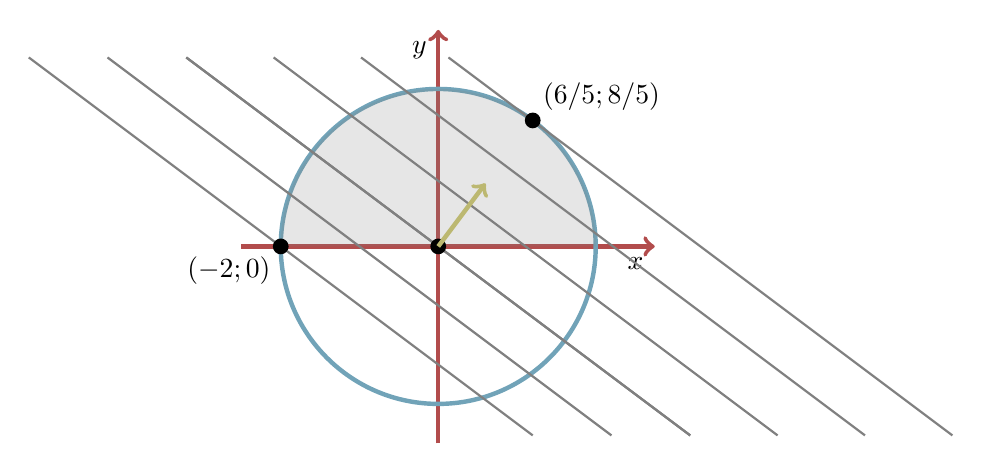
\begin{tikzpicture}[thick]
  \draw[-to, draw=red!40!gray, ultra thick]
  (-2.5, 0) -- (2.75, 0) node[below left] {$x$};
  \draw[-to, draw=red!40!gray, ultra thick]
  (0, -2.5) -- (0, 2.75) node[below left] {$y$};

  \draw[draw=cyan!40!gray, ultra thick] (0,0) circle (2);
  \fill[gray, opacity=.2] (2,0) arc [
      start angle=0,
      end angle=180,
      x radius=2cm,
      y radius=2cm,
    ];
  \foreach \s in {-2,-1,...,0}{
      \draw[
        xshift=\s*1cm,
        gray,
      ](-3.2,2.4) -- (3.2,-2.4);
    }
  \foreach \s in {0,1,...,3}{
      \draw[
        xshift=\s*1.11cm,
        gray,
      ](-3.2,2.4) -- (3.2,-2.4);
    }

  \fill (0,0) circle (.1);
  \fill (-2,0) circle (.1) node[below left] {$(-2;0)$};
  \fill (1.2,1.6) circle (.1) node[above right] {$(6/5;8/5)$};;

  \draw[ultra thick, -to, yellow!40!gray] (0,0) -- (.6,.8);
\end{tikzpicture}

\end{document}
